% 第二章:导数与微分
\chapter{导数与微分}
\section{导数的定义}
\begin{example}{}{}
    已知$x,y>0$,且$x^2+9y^2=12$,则$\dfrac{x+2}{y+1}-3x$的最小值为\underline{\hspace{2cm}}.
\end{example}
\begin{example}{}{}
    本题认为地球绕日轨道为正圆。现有一个半径是日地距离的一万分之一,且整个行星可以看成均匀球体。在该行星上诞生了两个文明:分别是在南极的冻成狗文明和在赤道的热成狗文明。两个文明之间为了友好往来,决定在它们的首都(分别在南极和赤道上)之间挖一条地下光滑隧道:摩擦力可以忽略的球形地铁可以纯粹在行星的引力的作用下从隧道一端滑行至另一端。两个文明的工程师们进行了详细的计算和规划,使得地铁往返于两个首都之间的时间达到最短。
    
    问:地铁每次单程运行时间是几个小时?(结果保留5位有效数字)
    
    提示:欧拉-拉格朗日方程;忽略行星自转:地球公转周期取365天
\end{example}
\text{d}
% 图片插入示例(注释掉,避免报错)
% \begin{figure}[htbp]
%     \centering
%     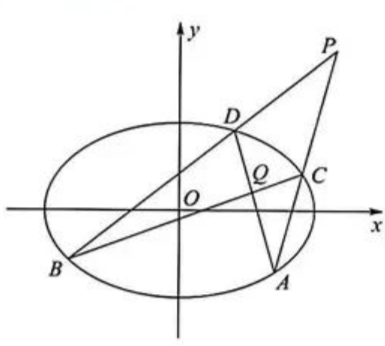
\includegraphics[width=0.6\textwidth]{flg/example.png}
%     \caption{导数的几何意义}
%     \label{fig:derivative}
% \end{figure}